\documentclass{article}\usepackage[]{graphicx}\usepackage[]{color}
%% maxwidth is the original width if it is less than linewidth
%% otherwise use linewidth (to make sure the graphics do not exceed the margin)
\makeatletter
\def\maxwidth{ %
  \ifdim\Gin@nat@width>\linewidth
    \linewidth
  \else
    \Gin@nat@width
  \fi
}
\makeatother

\definecolor{fgcolor}{rgb}{0.345, 0.345, 0.345}
\newcommand{\hlnum}[1]{\textcolor[rgb]{0.686,0.059,0.569}{#1}}%
\newcommand{\hlstr}[1]{\textcolor[rgb]{0.192,0.494,0.8}{#1}}%
\newcommand{\hlcom}[1]{\textcolor[rgb]{0.678,0.584,0.686}{\textit{#1}}}%
\newcommand{\hlopt}[1]{\textcolor[rgb]{0,0,0}{#1}}%
\newcommand{\hlstd}[1]{\textcolor[rgb]{0.345,0.345,0.345}{#1}}%
\newcommand{\hlkwa}[1]{\textcolor[rgb]{0.161,0.373,0.58}{\textbf{#1}}}%
\newcommand{\hlkwb}[1]{\textcolor[rgb]{0.69,0.353,0.396}{#1}}%
\newcommand{\hlkwc}[1]{\textcolor[rgb]{0.333,0.667,0.333}{#1}}%
\newcommand{\hlkwd}[1]{\textcolor[rgb]{0.737,0.353,0.396}{\textbf{#1}}}%
\let\hlipl\hlkwb

\usepackage{framed}
\makeatletter
\newenvironment{kframe}{%
 \def\at@end@of@kframe{}%
 \ifinner\ifhmode%
  \def\at@end@of@kframe{\end{minipage}}%
  \begin{minipage}{\columnwidth}%
 \fi\fi%
 \def\FrameCommand##1{\hskip\@totalleftmargin \hskip-\fboxsep
 \colorbox{shadecolor}{##1}\hskip-\fboxsep
     % There is no \\@totalrightmargin, so:
     \hskip-\linewidth \hskip-\@totalleftmargin \hskip\columnwidth}%
 \MakeFramed {\advance\hsize-\width
   \@totalleftmargin\z@ \linewidth\hsize
   \@setminipage}}%
 {\par\unskip\endMakeFramed%
 \at@end@of@kframe}
\makeatother

\definecolor{shadecolor}{rgb}{.97, .97, .97}
\definecolor{messagecolor}{rgb}{0, 0, 0}
\definecolor{warningcolor}{rgb}{1, 0, 1}
\definecolor{errorcolor}{rgb}{1, 0, 0}
\newenvironment{knitrout}{}{} % an empty environment to be redefined in TeX

\usepackage{alltt}
\title{Problem Set 8}
\author{Cameron Adams}


\usepackage{float, hyperref}
\usepackage[margin = 1in]{geometry}
\usepackage{graphicx}
\usepackage{sectsty}
\usepackage{hyperref}
\usepackage{amsmath}
\IfFileExists{upquote.sty}{\usepackage{upquote}}{}
\begin{document}
%\SweaveOpts{concordance=TRUE}

\maketitle





%1
\section{Let’s consider importance sampling and explore ...}
%1a
\subsection{Does the tail of the Pareto decay more quickly or more slowly than that of an exponential distribution?}

The pareto distribution decays more slowly than the exponential distribution
%1b
\subsection{Suppose f is an exponential density with parameter value ...}


\begin{knitrout}
\definecolor{shadecolor}{rgb}{0.969, 0.969, 0.969}\color{fgcolor}\begin{kframe}
\begin{alltt}
\hlkwd{rm}\hlstd{(}\hlkwc{list}\hlstd{=}\hlkwd{ls}\hlstd{())}

\hlkwd{require}\hlstd{(extraDistr)}

\hlcom{# parms}
\hlstd{m} \hlkwb{<-} \hlnum{10000}
\hlstd{a} \hlkwb{<-} \hlnum{3}
\hlstd{b} \hlkwb{<-} \hlnum{2}

\hlcom{#generate x according to parato}
\hlstd{x} \hlkwb{<-} \hlkwd{rpareto}\hlstd{(m,} \hlkwc{a} \hlstd{= a,} \hlkwc{b} \hlstd{= b)}

\hlcom{#generate f(x)}
\hlstd{f} \hlkwb{<-} \hlkwd{ifelse}\hlstd{(x} \hlopt{<} \hlnum{2}\hlstd{,} \hlnum{0}\hlstd{,} \hlkwd{dexp}\hlstd{(x} \hlopt{-} \hlnum{2}\hlstd{))}

\hlcom{#generate g(x)}
\hlstd{g} \hlkwb{<-} \hlkwd{dpareto}\hlstd{(x,} \hlkwc{a} \hlstd{= a,} \hlkwc{b} \hlstd{= b)}

\hlcom{#check g(x) satisfies paraeto conditions}
\hlkwd{sum}\hlstd{(g} \hlopt{>} \hlnum{2} \hlopt{&} \hlstd{g} \hlopt{<} \hlnum{1e9}\hlstd{)}
\end{alltt}
\begin{verbatim}
## [1] 0
\end{verbatim}
\begin{alltt}
\hlcom{#h(x) = h * f / g}
\hlstd{h_x} \hlkwb{<-} \hlstd{x}\hlopt{*}\hlstd{f}\hlopt{/}\hlstd{g} \hlcom{# x}
\hlstd{h_x2} \hlkwb{<-} \hlstd{x}\hlopt{^}\hlnum{2}\hlopt{*}\hlstd{f}\hlopt{/}\hlstd{g} \hlcom{# x^2}

\hlcom{#get expection}
\hlkwd{mean}\hlstd{(h_x)}
\end{alltt}
\begin{verbatim}
## [1] 2.998046
\end{verbatim}
\begin{alltt}
\hlkwd{mean}\hlstd{(h_x2)}
\end{alltt}
\begin{verbatim}
## [1] 10.05176
\end{verbatim}
\begin{alltt}
\hlcom{#histograms}
\hlstd{par_default} \hlkwb{<-} \hlkwd{par}\hlstd{(}\hlkwc{no.readonly} \hlstd{=} \hlnum{TRUE}\hlstd{)}
\hlkwd{par}\hlstd{(}\hlkwc{mfrow} \hlstd{=} \hlkwd{c}\hlstd{(}\hlnum{2}\hlstd{,} \hlnum{2}\hlstd{),} \hlkwc{oma} \hlstd{=} \hlkwd{c}\hlstd{(}\hlnum{0}\hlstd{,} \hlnum{0}\hlstd{,} \hlnum{2}\hlstd{,} \hlnum{0}\hlstd{))}
\hlkwd{hist}\hlstd{(h_x,} \hlkwc{main} \hlstd{=} \hlstr{"x f(x) / g(x)"}\hlstd{)}
\hlkwd{hist}\hlstd{(f} \hlopt{/} \hlstd{g,} \hlkwc{main} \hlstd{=} \hlstr{"f(x)/g(x)"}\hlstd{)}
\hlkwd{hist}\hlstd{(h_x2,} \hlkwc{main} \hlstd{=} \hlstr{"x^2 f(x) / g(x)"}\hlstd{)}
\hlkwd{mtext}\hlstd{(}\hlkwc{outer} \hlstd{= T,} \hlkwc{text} \hlstd{=} \hlstr{"Problem 1b"}\hlstd{,} \hlkwc{font} \hlstd{=} \hlnum{2}\hlstd{)}
\hlkwd{par}\hlstd{(par_default)}
\end{alltt}
\end{kframe}
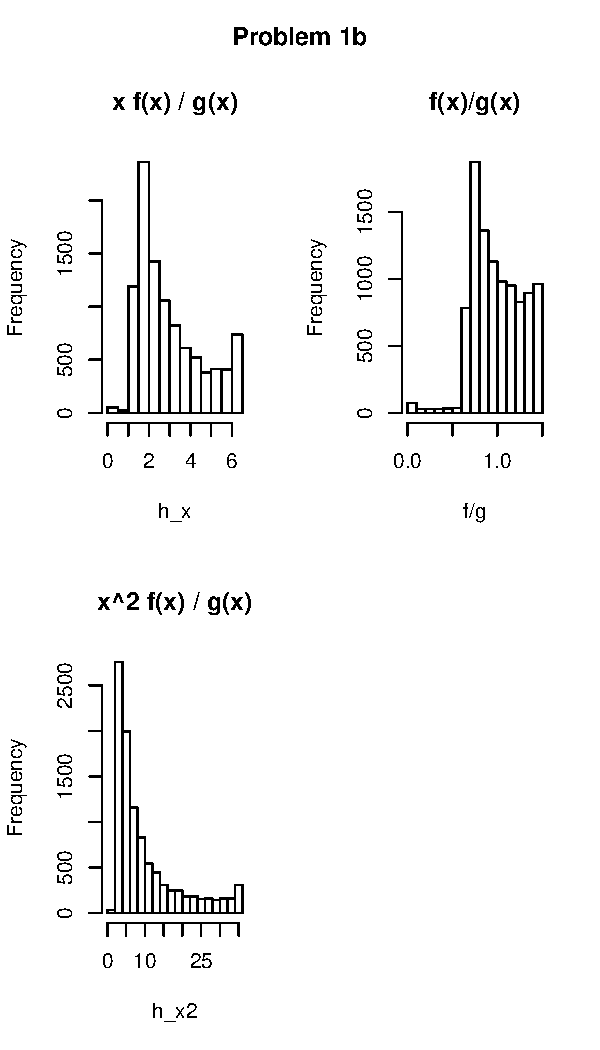
\includegraphics[width=\maxwidth]{figure/unnamed-chunk-2-1} 

\end{knitrout}

It appears that large x values have very small weights and x values approaching 2 will have large weights
%1c
\subsection{Now suppose f is the Pareto distribution described above and our sampling...}

\begin{knitrout}
\definecolor{shadecolor}{rgb}{0.969, 0.969, 0.969}\color{fgcolor}\begin{kframe}
\begin{alltt}
\hlcom{#generate x and f}
\hlstd{x} \hlkwb{<-} \hlkwd{rexp}\hlstd{(m)}\hlopt{+}\hlnum{2} \hlcom{#exp}
\hlstd{f} \hlkwb{<-} \hlkwd{dpareto}\hlstd{(x, a, b)} \hlcom{#pareto}

\hlcom{#generate g}
\hlstd{g} \hlkwb{<-} \hlkwd{ifelse}\hlstd{(x}\hlopt{<}\hlnum{2}\hlstd{,} \hlnum{0}\hlstd{,} \hlkwd{dexp}\hlstd{(x}\hlopt{-}\hlnum{2}\hlstd{))}
\hlstd{h_x} \hlkwb{<-} \hlstd{x}\hlopt{*}\hlstd{f}\hlopt{/}\hlstd{g}
\hlstd{h_x2} \hlkwb{<-} \hlstd{x}\hlopt{^}\hlnum{2}\hlopt{*}\hlstd{f}\hlopt{/}\hlstd{g}

\hlcom{#get expection}
\hlkwd{mean}\hlstd{(h_x)}
\end{alltt}
\begin{verbatim}
## [1] 2.943074
\end{verbatim}
\begin{alltt}
\hlkwd{mean}\hlstd{(h_x2)}
\end{alltt}
\begin{verbatim}
## [1] 10.48022
\end{verbatim}
\begin{alltt}
\hlcom{#histograms}
\hlkwd{par}\hlstd{(}\hlkwc{mfrow} \hlstd{=} \hlkwd{c}\hlstd{(}\hlnum{2}\hlstd{,} \hlnum{2}\hlstd{),} \hlkwc{oma} \hlstd{=} \hlkwd{c}\hlstd{(}\hlnum{0}\hlstd{,} \hlnum{0}\hlstd{,} \hlnum{2}\hlstd{,} \hlnum{0}\hlstd{))}
\hlkwd{hist}\hlstd{(h_x,} \hlkwc{main} \hlstd{=} \hlstr{"Histogram of x f(x) / g(x)"}\hlstd{)}
\hlkwd{hist}\hlstd{(f} \hlopt{/} \hlstd{g,} \hlkwc{main} \hlstd{=} \hlstr{"Histogram of f(x)/g(x)"}\hlstd{)}
\hlkwd{hist}\hlstd{(h_x2,} \hlkwc{main} \hlstd{=} \hlstr{"Histogram of x^2 f(x) / g(x)"}\hlstd{)}
\hlkwd{mtext}\hlstd{(}\hlkwc{outer} \hlstd{= T,} \hlkwc{text} \hlstd{=} \hlstr{"Problem 1c"}\hlstd{,} \hlkwc{font} \hlstd{=} \hlnum{2}\hlstd{)}
\hlkwd{par}\hlstd{(par_default)}
\end{alltt}
\end{kframe}
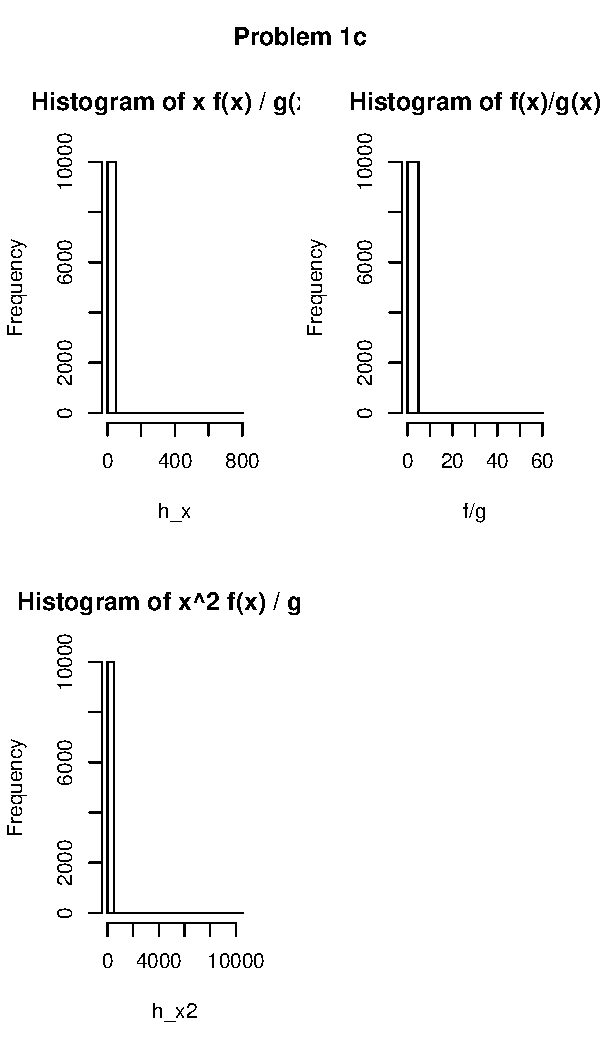
\includegraphics[width=\maxwidth]{figure/unnamed-chunk-3-1} 

\end{knitrout}
The version of smapling will have large weights for values close 0, and smaller weights to values close to 0, with no/zero weight with values > 2.

%2
\section{Consider the “helical valley” function ...}

\begin{knitrout}
\definecolor{shadecolor}{rgb}{0.969, 0.969, 0.969}\color{fgcolor}\begin{kframe}
\begin{alltt}
\hlkwd{source}\hlstd{()}
\end{alltt}


{\ttfamily\noindent\bfseries\color{errorcolor}{\#\# Error in source(): argument "{}file"{} is missing, with no default}}\begin{alltt}
\hlstd{theta} \hlkwb{<-} \hlkwa{function}\hlstd{(}\hlkwc{x1}\hlstd{,}\hlkwc{x2}\hlstd{)} \hlkwd{atan2}\hlstd{(x2, x1)}\hlopt{/}\hlstd{(}\hlnum{2}\hlopt{*}\hlstd{pi)}

\hlstd{f} \hlkwb{<-} \hlkwa{function}\hlstd{(}\hlkwc{x}\hlstd{) \{}
  \hlstd{f1} \hlkwb{<-} \hlnum{10}\hlopt{*}\hlstd{(x[}\hlnum{3}\hlstd{]} \hlopt{-} \hlnum{10}\hlopt{*}\hlkwd{theta}\hlstd{(x[}\hlnum{1}\hlstd{],x[}\hlnum{2}\hlstd{]))}
  \hlstd{f2} \hlkwb{<-} \hlnum{10}\hlopt{*}\hlstd{(}\hlkwd{sqrt}\hlstd{(x[}\hlnum{1}\hlstd{]}\hlopt{^}\hlnum{2} \hlopt{+} \hlstd{x[}\hlnum{2}\hlstd{]}\hlopt{^}\hlnum{2}\hlstd{)} \hlopt{-} \hlnum{1}\hlstd{)}
  \hlstd{f3} \hlkwb{<-} \hlstd{x[}\hlnum{3}\hlstd{]}
  \hlkwd{return}\hlstd{(f1}\hlopt{^}\hlnum{2} \hlopt{+} \hlstd{f2}\hlopt{^}\hlnum{2} \hlopt{+} \hlstd{f3}\hlopt{^}\hlnum{2}\hlstd{)}
\hlstd{\}}

\hlkwd{source}\hlstd{(}\hlstr{"./ps8.R"}\hlstd{)}

\hlcom{#generate x1 and x2}
\hlstd{x1} \hlkwb{<-} \hlstd{x2} \hlkwb{<-} \hlkwd{seq}\hlstd{(}\hlopt{-}\hlnum{10}\hlstd{,} \hlnum{10}\hlstd{,} \hlkwc{length.out} \hlstd{= n)}
\hlstd{x} \hlkwb{<-} \hlkwd{cbind}\hlstd{(}\hlkwd{expand.grid}\hlstd{(x1, x2),} \hlnum{0}\hlstd{)}

\hlcom{#x3 = 0}
\hlstd{x} \hlkwb{<-} \hlkwd{cbind}\hlstd{(}\hlkwd{expand.grid}\hlstd{(x1, x2),} \hlnum{0}\hlstd{)}
\hlstd{x3_0}    \hlkwb{<-} \hlkwd{matrix}\hlstd{(}\hlkwd{apply}\hlstd{(}\hlkwd{cbind}\hlstd{(}\hlkwd{expand.grid}\hlstd{(x1, x2),} \hlnum{0}\hlstd{),} \hlnum{1}\hlstd{, f),} \hlkwc{ncol} \hlstd{= n)}
\hlstd{x3_5}    \hlkwb{<-} \hlkwd{matrix}\hlstd{(}\hlkwd{apply}\hlstd{(}\hlkwd{cbind}\hlstd{(}\hlkwd{expand.grid}\hlstd{(x1, x2),} \hlnum{5}\hlstd{),} \hlnum{1}\hlstd{, f),} \hlkwc{ncol} \hlstd{= n)}
\hlstd{x3_neg5} \hlkwb{<-} \hlkwd{matrix}\hlstd{(}\hlkwd{apply}\hlstd{(}\hlkwd{cbind}\hlstd{(}\hlkwd{expand.grid}\hlstd{(x1, x2),} \hlopt{-}\hlnum{5}\hlstd{),} \hlnum{1}\hlstd{, f),} \hlkwc{ncol} \hlstd{= n)}
\hlstd{x3_10}   \hlkwb{<-} \hlkwd{matrix}\hlstd{(}\hlkwd{apply}\hlstd{(}\hlkwd{cbind}\hlstd{(}\hlkwd{expand.grid}\hlstd{(x1, x2),} \hlnum{10}\hlstd{),} \hlnum{1}\hlstd{, f),} \hlkwc{ncol} \hlstd{= n)}

\hlcom{#plot contours}
\hlkwd{par}\hlstd{(}\hlkwc{mfrow} \hlstd{=} \hlkwd{c}\hlstd{(}\hlnum{2}\hlstd{,} \hlnum{2}\hlstd{))}
\hlkwd{contour}\hlstd{(x1, x2, x3_0,} \hlkwc{main} \hlstd{=} \hlstr{"x3 = 0"}\hlstd{)}
\hlkwd{contour}\hlstd{(x1, x2, x3_5,} \hlkwc{main} \hlstd{=} \hlstr{"x3 = 5"}\hlstd{)}
\hlkwd{contour}\hlstd{(x1, x2, x3_neg5,} \hlkwc{main} \hlstd{=} \hlstr{"x3 = -5"}\hlstd{)}
\hlkwd{contour}\hlstd{(x1, x2, x3_10,} \hlkwc{main} \hlstd{=} \hlstr{"x3 = 10"}\hlstd{)}
\end{alltt}
\end{kframe}
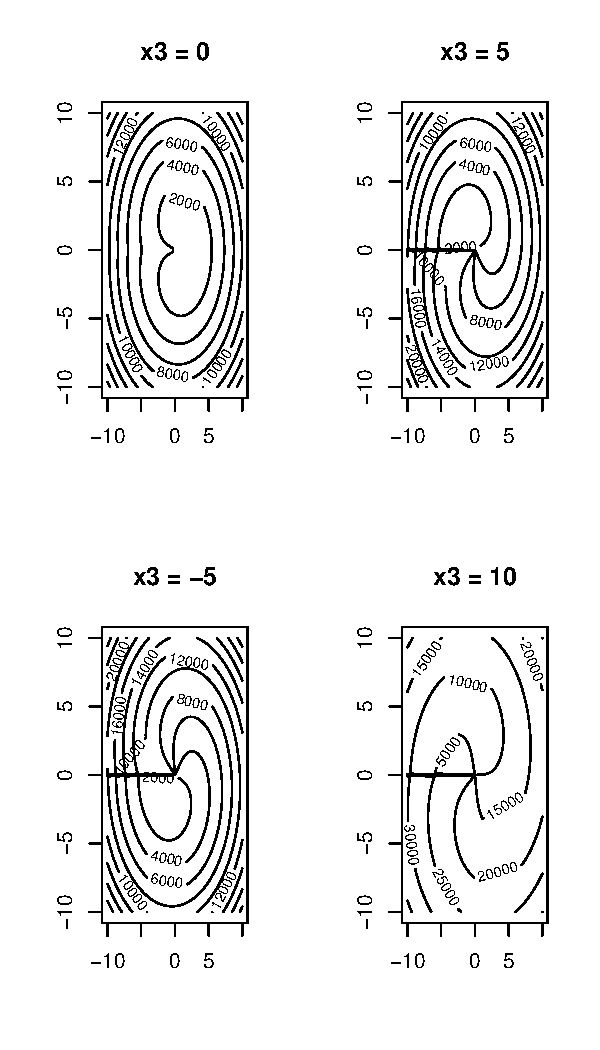
\includegraphics[width=\maxwidth]{figure/unnamed-chunk-4-1} 
\begin{kframe}\begin{alltt}
\hlkwd{par}\hlstd{(par_default)}

\hlcom{#plot 3d}
\hlkwd{par}\hlstd{(}\hlkwc{mfrow}\hlstd{=}\hlkwd{c}\hlstd{(}\hlnum{2}\hlstd{,} \hlnum{2}\hlstd{),} \hlkwc{mar} \hlstd{=} \hlkwd{c}\hlstd{(}\hlnum{3}\hlstd{,} \hlnum{0}\hlstd{,} \hlnum{1}\hlstd{,} \hlnum{0}\hlstd{))}
\hlkwd{persp}\hlstd{(x1, x2, x3_0,}\hlkwc{main} \hlstd{=} \hlstr{"x3 = 0"}\hlstd{)}
\hlkwd{persp}\hlstd{(x1, x2, x3_5,} \hlkwc{main} \hlstd{=} \hlstr{"x3 = 5"}\hlstd{)}
\hlkwd{persp}\hlstd{(x1, x2, x3_neg5,} \hlkwc{main} \hlstd{=} \hlstr{"x3 = -5"}\hlstd{)}
\hlkwd{persp}\hlstd{(x1, x2, x3_10,} \hlkwc{main} \hlstd{=} \hlstr{"x3 = 10"}\hlstd{)}
\end{alltt}
\end{kframe}
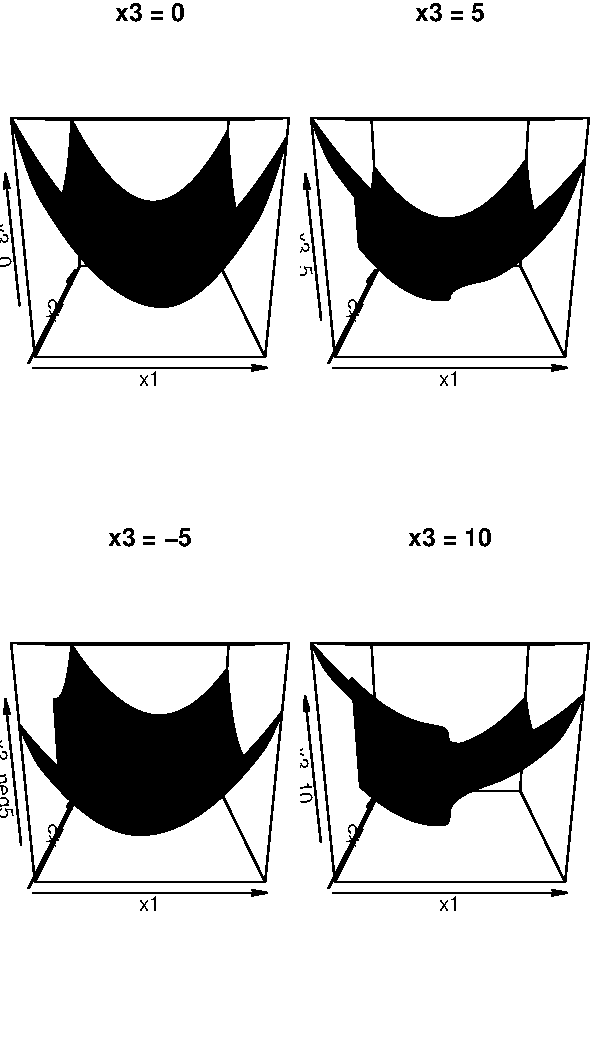
\includegraphics[width=\maxwidth]{figure/unnamed-chunk-4-2} 
\begin{kframe}\begin{alltt}
\hlkwd{par}\hlstd{(par_default)}

\hlcom{#optim}
\hlkwd{optim}\hlstd{(}\hlkwc{par} \hlstd{=} \hlkwd{c}\hlstd{(}\hlnum{0}\hlstd{,} \hlnum{0}\hlstd{,} \hlnum{0}\hlstd{),} \hlkwc{fn} \hlstd{= f)[}\hlnum{1}\hlopt{:}\hlnum{2}\hlstd{]}
\end{alltt}
\begin{verbatim}
## $par
## [1] 0.999978292 0.002730698 0.004284640
## 
## $value
## [1] 1.876851e-05
\end{verbatim}
\begin{alltt}
\hlkwd{optim}\hlstd{(}\hlkwc{par} \hlstd{=} \hlkwd{c}\hlstd{(}\hlnum{1}\hlstd{,} \hlnum{1}\hlstd{,} \hlnum{1}\hlstd{),} \hlkwc{fn} \hlstd{= f)[}\hlnum{1}\hlopt{:}\hlnum{2}\hlstd{]}
\end{alltt}
\begin{verbatim}
## $par
## [1]  0.9999779414 -0.0001349269 -0.0001927127
## 
## $value
## [1] 1.343098e-07
\end{verbatim}
\begin{alltt}
\hlkwd{optim}\hlstd{(}\hlkwc{par} \hlstd{=} \hlkwd{c}\hlstd{(}\hlnum{20}\hlstd{,} \hlnum{100}\hlstd{,} \hlnum{1e5}\hlstd{),} \hlkwc{fn} \hlstd{= f)[}\hlnum{1}\hlopt{:}\hlnum{2}\hlstd{]}
\end{alltt}
\begin{verbatim}
## $par
## [1]  -4.096157 -11.468532   3.170776
## 
## $value
## [1] 16369.8
\end{verbatim}
\begin{alltt}
\hlkwd{optim}\hlstd{(}\hlkwc{par} \hlstd{=} \hlkwd{c}\hlstd{(}\hlnum{20}\hlstd{,} \hlnum{100}\hlstd{,} \hlnum{1e5}\hlstd{),} \hlkwc{fn} \hlstd{= f,} \hlkwc{method} \hlstd{=} \hlstr{"BFGS"}\hlstd{)[}\hlnum{1}\hlopt{:}\hlnum{2}\hlstd{]}
\end{alltt}
\begin{verbatim}
## $par
## [1] 1.000000e+00 5.252510e-10 8.400998e-10
## 
## $value
## [1] 7.099825e-19
\end{verbatim}
\begin{alltt}
\hlkwd{optim}\hlstd{(}\hlkwc{par} \hlstd{=} \hlkwd{c}\hlstd{(}\hlopt{-}\hlnum{100}\hlstd{,} \hlopt{-}\hlnum{1000}\hlstd{,} \hlopt{-}\hlnum{1e5}\hlstd{),} \hlkwc{fn} \hlstd{= f)[}\hlnum{1}\hlopt{:}\hlnum{2}\hlstd{]}
\end{alltt}
\begin{verbatim}
## $par
## [1] -4.771779 -6.296438 -6.561802
## 
## $value
## [1] 5722.384
\end{verbatim}
\begin{alltt}
\hlkwd{optim}\hlstd{(}\hlkwc{par} \hlstd{=} \hlkwd{c}\hlstd{(}\hlopt{-}\hlnum{100}\hlstd{,} \hlopt{-}\hlnum{1000}\hlstd{,} \hlopt{-}\hlnum{1e5}\hlstd{),} \hlkwc{fn} \hlstd{= f,} \hlkwc{method} \hlstd{=} \hlstr{"BFGS"}\hlstd{)[}\hlnum{1}\hlopt{:}\hlnum{2}\hlstd{]}
\end{alltt}
\begin{verbatim}
## $par
## [1] 1.000000e+00 1.880569e-13 3.056140e-13
## 
## $value
## [1] 1.215431e-25
\end{verbatim}
\begin{alltt}
\hlcom{#nlm}
\hlkwd{nlm}\hlstd{(f,} \hlkwc{p} \hlstd{=} \hlkwd{c}\hlstd{(}\hlnum{0}\hlstd{,} \hlnum{0}\hlstd{,} \hlnum{0}\hlstd{))[}\hlnum{1}\hlopt{:}\hlnum{2}\hlstd{]}
\end{alltt}
\begin{verbatim}
## $minimum
## [1] 100
## 
## $estimate
## [1] 0 0 0
\end{verbatim}
\begin{alltt}
\hlkwd{nlm}\hlstd{(f,} \hlkwc{p} \hlstd{=} \hlkwd{c}\hlstd{(}\hlnum{1}\hlstd{,} \hlnum{1}\hlstd{,} \hlnum{1}\hlstd{))[}\hlnum{1}\hlopt{:}\hlnum{2}\hlstd{]}
\end{alltt}
\begin{verbatim}
## $minimum
## [1] 1.702065e-08
## 
## $estimate
## [1]  9.999995e-01 -8.225859e-05 -1.301257e-04
\end{verbatim}
\begin{alltt}
\hlkwd{nlm}\hlstd{(f,} \hlkwc{p} \hlstd{=} \hlkwd{c}\hlstd{(}\hlnum{20}\hlstd{,} \hlnum{100}\hlstd{,} \hlnum{1e5}\hlstd{))[}\hlnum{1}\hlopt{:}\hlnum{2}\hlstd{]}
\end{alltt}
\begin{verbatim}
## $minimum
## [1] 2.140881e-17
## 
## $estimate
## [1]  1.000000e+00 -9.779836e-11  2.902313e-10
\end{verbatim}
\begin{alltt}
\hlkwd{nlm}\hlstd{(f,} \hlkwc{p} \hlstd{=} \hlkwd{c}\hlstd{(}\hlopt{-}\hlnum{100}\hlstd{,} \hlopt{-}\hlnum{1000}\hlstd{,} \hlopt{-}\hlnum{1e5}\hlstd{))[}\hlnum{1}\hlopt{:}\hlnum{2}\hlstd{]}
\end{alltt}
\begin{verbatim}
## $minimum
## [1] 1.674813e-16
## 
## $estimate
## [1] 1.000000e+00 1.451395e-09 3.037370e-09
\end{verbatim}
\end{kframe}
\end{knitrout}

I plotted the provided "helical valley" function using constant values of x3 to get slices of x1 and x2. From the plots, it looks like there will be local minima, and there are valleyes throughout the function. 

The results from the opimizataions using optim() and nlm() indicate that there are indeed local minima. When using non-ideal non-scaled starting values, both optim and nlm converge to solutions that are incorrect. NLM performs better than optim with "Nelder-Mead" and "BFGS". 

%3
\section{Consider a censored regression problem. We assume ...}

\subsection{Design an EM algorithm to estimate the 3 parameters, θ = (β0, β1, σ2
), taking ...}


$X:$ covariates
$Y:$ outcome
$Z:$ values of censored Y values

Likelihood function:
$$\begin{aligned}
\mathcal{L}(\theta; X, Y, Z) &= \prod_{i=1}^c \frac{1}{\sqrt{2\pi\sigma^2}} exp(-\frac{1}{2\sigma^2} (z_i - (\beta_0 + \beta_1 x_i))^2) \prod_{j=c+1}^n  \frac{1}{\sqrt{2\sigma^2}}   exp(-\frac{1}{2\sigma^2} (y_i - (\beta_0 + \beta_1 x_j))^2) \\
&= (\frac{1}{\sqrt{2\pi\sigma^2}})^n \prod_{i=1}^c  exp(-\frac{1}{2\sigma^2} (z_i - (\beta_0 + \beta_1 x_i))^2) \prod_{j=c+1}^n     exp(-\frac{1}{2\sigma^2} (y_i - (\beta_0 + \beta_1 x_j))^2)) \\
\end{aligned}$$

log-Likelihood function:
$$\begin{aligned}
\ell(\theta;X,Y,Z)=& -\frac{n}{2} log(2\pi \sigma^2) - \frac{1}{2\sigma^2} \sum^c_{i=1} (z_i - (\beta_0 + \beta_1x_i))^2 - \frac{1}{2\sigma^2} \sum^n_{j=c+1} (y_i - (\beta_0 + \beta_1x_j))^2 \\
=& -\frac{n}{2}log(2\pi\sigma^2) - \frac{1}{2\sigma^2} \sum_{j=c+1}^n \sum^n_{j=c+1} (y_i - (\beta_0 + \beta_1x_j))^2 \\
&- \frac{1}{2\sigma^2} \sum^c_{i=1} (z_i^2 - 2z_i (\beta_0 + \beta_1 x_i) + (\beta_0 + \beta_1x_i)^2) \\
\end{aligned}$$

Expectations and variance:
$$\begin{aligned}
E[\tau^*|X,Y,\theta_t] &= \frac{1}{\sigma_t}  (\tau - (\beta_{0,t} + \beta_{1,t}x_i)) \\
E[\rho(\tau^*) |X,Y,\theta_t] &= \frac{\phi(\tau^*)}{(1-\Phi(\tau^*)^2)} \\
E[z_i|X,Y,\theta_t] &= (\beta_{0,t} + \beta_{1,t}x_i) + \sigma_t\rho(\tau^*) \\
var(z_i | X,Y,\theta_t) &= \sigma^2_t (1 + \tau^* \rho (\tau^*) - \rho(\tau^*)^2)
\end{aligned}$$



$Q$ function:
$$\begin{aligned}
Q(\theta | \theta_t)&= E[\ell(\theta; X, Y, Z)|X,Y, \theta_t] \\
=& -\frac{n}{2} log(2 \pi \sigma^2) - \frac{1}{2\sigma^2} \sum^n_{j=c+1}(y_i - (\beta_0 + \beta_1x_j))^2 \\
&+ -\frac{1}{2\sigma^2} \sum^c_{i=1}(E[z^2_i | X,Y,\theta_t] - 2E[z_i|X,Y,\theta_t](\beta_0 + \beta_1x_i) + (\beta_0 + \beta_1x_i)^2 )\\
=& -\frac{n}{2} log(2\pi\sigma^2) - \frac{1}{2\sigma^2} \sum_{j=c+1}^n (y_i - (\beta_0 + \beta_1x_j))^2  \\
&- \frac{1}{2\sigma^2} \sum_{i=1}^c (E[z_i|X,Y,\theta_t] - (\beta_0 + \beta_1x_i))^2 + \sum_{i=1}^c var(z_i|X,Y,\theta_t) 
\end{aligned}$$

Partial derivative for $\beta_0$
$$\begin{aligned}
\frac{\partial}{\partial \beta_0} Q(\theta|\theta_t)  =& -\frac{1}{2\sigma^2} \sum_{j=c+1}^n 2(y_i - (\beta_0 + \beta_1x_j))(-1) - \frac{1}{2\sigma^2} \sum_{i=1}^c 2(E[z_i|X,Y,\theta_t] - (\beta_0 + \beta_1 x_i)) (-1) \\
=& \frac{1}{\sigma^2} (\sum_{j=c+1}^n(y_j - \beta_1x_j) - \sum_{j=c+1}^n \beta_0 + \sum_{i=1}^c (E[z_i|X,Y,\theta_t] - \beta_1x_i) - \sum_{i=1}^c\beta_o) \\
=& \frac{1}{\sigma^2} (\sum^n_{j=c+1} (y_j - \beta_1x_j) - \sum_{i=1}^c (E[z_i|X,Y,\theta_t] - \beta_1x_i) - n\beta_0) \\
=& 0 \\
\text{solve for } \beta_0 & \\
\hat{\beta_0} &= \frac{1}{n} (\sum^n_{j = c+1} (y-\beta_1 x_j) + \sum_{i=1}^c (E[z_i|X,Y,\theta_t] - \beta_1 x_i))
\end{aligned}$$

Partial derivative for $\beta_1$
$$\begin{aligned}
\frac{\partial}{\partial \beta_1} Q(\theta|\theta_t)  =&- \frac{1}{2\sigma^2} \sum_{j=c+1}^n 2(y_i - (\beta_0 + \beta_1x_j))(-x_j) - \frac{1}{2\sigma^2} \sum_{i=1}^c 2(E[z_i | X,Y,\theta_t] - (\beta_0 + \beta_1x_i)) (-x_i) \\
=& \frac{1}{\sigma^2} (\sum_{j=c+1}^n x_j (y_j - \beta_0)- \sum^n_{j=c+1} \beta_1 x_j^2 + \sum_{i=1}^c x_i (E[z_i | X,Y,\theta_t] - \beta_0) - \sum_{i=1}^c \beta_1 x_i^2) \\
=& \frac{1}{\sigma^2} (\sum^n_{j=c+1} x_j(y_j-\beta_0) + \sum_{i=1}^c x_i(E[z_i|X,Y,\theta_t] - \beta_0 ) - \beta_1 \sum_{k=1}^n x_k^2) \\
=& 0 \\
\text{solve for }\beta_1 &\\
\hat{\beta_1} =& \frac{1}{\sum_{k=1}^nx_k^2} (\sum_{j=c+1}^n x_j (y_j - \beta_0) + \sum_{i=1}^c x_i(E[z_i|X,Y,\theta_t] - \beta_0))
\end{aligned}$$

Partial derivative for $\sigma^2$
$$\begin{aligned}
\frac{\partial}{\partial \sigma^2} Q(\theta|\theta_t)  =& -\frac{n}{2} (\frac{1}{2 \pi\sigma^2})(2\pi) + \frac{1}{2\sigma^4} \sum^n_{j=c+1} (y_j - (\beta_0 + \beta_1 x_j))^2 \\
&+ \frac{1}{2\sigma^4} \sum_{i=1}^c (E[z_i|X,Y,\theta_t] - (\beta_0 + \beta_1x_i))^2 + \frac{1}{2\sigma^4} \sum_{i=1}^c var(z_i|X,Y,\theta_t) \\
=& \frac{1}{2\sigma^4} (n\sigma^2 + \sum_{j=c+1}^n (y_i - (\beta_0 + \beta_1x_j))^2 ) \\
&+ \sum_{i=1}^c (E[z_i|X,Y,\sigma^t] - (\beta_0 + \beta_1x_i)) + \sum_{i=1}^c var(z_i|X,Y,\theta_t) \\
=&0 \\
\text{solve for } \sigma^2 &\\
\hat{sigma^2} =& \frac{1}{n} (\sum^n_{j=c+1}(y_j - (\beta_0 + \beta_1x_j))^2 + \sum_{i=1}^c (E[z_i | X,Y,\theta_t] - (\beta_0 + \beta_1x_i))^2 + \sum_{i=1}^c var(z_i|X,Y,\theta_t))
\end{aligned}$$

The $\sigma^2$ estimator is a ratio with a numerator contains the normal sum of squares for the non-censored data and the sum of squares for teh cnesored data, the varaicne of teh imputed censored data using $\theta^t$.
%3.2
\subsection{Propose reasonable starting values for the 3 parameters...}

Using observed $Y_i$ values, if 
\begin{itemize}
\item $\bar{x} =   1 / (n - c) \sum_{j=c+1}^n$
\item $\bar{y} = 1 / (n-c) \sum_{j=c+1}^n y_j$
\end{itemize}
then:
$$\begin{aligned}
\hat{\beta}_{0,0} &= 1 / (n-c) \sum_{j=c+1}^n (y_j - \hat{\beta}_{1,0}x_j) \\
&... \\
 &= 1 / (n-c) \sum_{j=c+1}^n \bigg( y_j - x_j \frac{ \sum_{j=c+1}^n x_j(y_i - \bar{y})}{ \sum_{j=c+1}^n x_j(x_j - \bar{x}) } \bigg) 
\end{aligned}$$

$$\begin{aligned}
\hat{\beta}_{1,0} =& \frac{1}{ \sum_{j=c+1}^n x_j^2} \bigg( \sum_{j=c+1}^n (y_i - \hat{\beta}_{0,0})x_j \bigg) \\
\hat{\beta}_{1,0}  \sum_{j=c+1}^n x_j^2 =& \sum_{j=c+1}^n x_j (y_j - \frac{1}{n-c} \sum_{j=c+1}^n (y_j - \hat{\beta}_{1,0}x_j)) \\
=& \bigg(\sum_{j=c+1}^c x_j (y_j - \bar{y})\bigg)  - (\hat{\beta}_{1,0} \sum_{j=c+1}^n x_j \bar{x}) \\
\hat{\beta}_{1,0} \sum_{j=c+1}^n x_j (x_j - \bar{x}) = \sum_{j = c+1}^n x_j (y_j - \bar{y}) \\
\hat{\beta}_{1,0}  = &\frac{\sum_{j = c+1}^n x_j (y_j - \bar{y})}{\sum_{j=c+1}^n x_j (x_j - \bar{x})} 
\end{aligned}$$


$$\begin{aligned}
\hat{\sigma}^2_0 =& \frac{1}{n} \sum_{j=c+1}^n (y_j - (\hat{\beta}_{0,0} + \hat{\beta}_{1,0}x_j))^2
\end{aligned}$$

\subsection{Write an R function, with auxiliary functions as needed...}

EM function is below.
\begin{knitrout}
\definecolor{shadecolor}{rgb}{0.969, 0.969, 0.969}\color{fgcolor}\begin{kframe}
\begin{alltt}
\hlcom{#generate data}
\hlkwd{source}\hlstd{(}\hlstr{"./ps8.R"}\hlstd{)}

\hlcom{#########}
\hlcom{# EM function}
\hlcom{##########}

\hlstd{em} \hlkwb{=} \hlkwa{function}\hlstd{(}\hlkwc{x}\hlstd{,} \hlkwc{y}\hlstd{,} \hlkwc{tau}\hlstd{,} \hlkwc{stop}\hlstd{=}\hlnum{1000}\hlstd{,} \hlkwc{stopLike}\hlstd{=}\hlnum{1e-6}\hlstd{) \{} \hlcom{# x: vector of x_i values}
    \hlcom{#y = vector of y_i values, with NA for censored data}
    \hlcom{#x = observted covariates}
    \hlcom{#b0 = beta0}
    \hlcom{#b1 = beta1}
    \hlcom{#sigma2 = sigma^2}
    \hlcom{#ll = log Likelihood}
    \hlcom{#tau: threshold for y_i censoring}
    \hlcom{#stop: maximum number of iterations through EM algorithm}
    \hlcom{#stopLike: diff of loglik of parameters of iterations }
        \hlcom{#returns: data frame of (b_0, b_1, s^2, loglik) for each iteration}

    \hlcom{#set output df  }
    \hlstd{results} \hlkwb{<-} \hlkwd{data.frame}\hlstd{(}\hlkwd{matrix}\hlstd{(}\hlnum{NA}\hlstd{,} \hlkwc{nrow}\hlstd{=stop,} \hlkwc{ncol} \hlstd{=} \hlnum{4}\hlstd{))}
    \hlkwd{names}\hlstd{(results)} \hlkwb{<-}  \hlkwd{c}\hlstd{(}\hlstr{"b0"}\hlstd{,} \hlstr{"b1"}\hlstd{,} \hlstr{"sigma2"}\hlstd{,} \hlstr{"ll"}\hlstd{)}

    \hlcom{#init parms }
    \hlstd{missing} \hlkwb{<-} \hlkwd{is.na}\hlstd{(y)}
    \hlstd{mod} \hlkwb{<-} \hlkwd{lm}\hlstd{(y} \hlopt{~} \hlstd{x)}
    \hlstd{results[}\hlnum{1}\hlstd{, ]} \hlkwb{<-} \hlkwd{c}\hlstd{(mod}\hlopt{$}\hlstd{coefficients,} \hlkwd{var}\hlstd{(mod}\hlopt{$}\hlstd{residuals),} \hlkwd{logLik}\hlstd{(mod)[[}\hlnum{1}\hlstd{]])}

    \hlkwa{for}\hlstd{(i} \hlkwa{in} \hlnum{2}\hlopt{:}\hlstd{stop) \{}

        \hlcom{#E-step: impute censored data}
        \hlstd{mu} \hlkwb{<-} \hlstd{results}\hlopt{$}\hlstd{b0[i} \hlopt{-} \hlnum{1}\hlstd{]} \hlopt{+} \hlstd{results}\hlopt{$}\hlstd{b1[i} \hlopt{-} \hlnum{1}\hlstd{]} \hlopt{*} \hlstd{x[missing]}
        \hlstd{tau_star} \hlkwb{<-} \hlstd{(tau} \hlopt{-} \hlstd{mu)} \hlopt{/} \hlkwd{sqrt}\hlstd{(results}\hlopt{$}\hlstd{sigma2[i} \hlopt{-} \hlnum{1}\hlstd{])}
        \hlstd{rho} \hlkwb{<-} \hlkwd{dnorm}\hlstd{(tau_star)} \hlopt{/} \hlstd{(}\hlnum{1} \hlopt{-} \hlkwd{pnorm}\hlstd{(tau_star))}
        \hlstd{y[missing]} \hlkwb{<-} \hlstd{mu} \hlopt{+} \hlkwd{sqrt}\hlstd{(results}\hlopt{$}\hlstd{sigma2[i} \hlopt{-} \hlnum{1}\hlstd{])} \hlopt{*} \hlstd{rho}
        \hlstd{var_z} \hlkwb{<-} \hlstd{results}\hlopt{$}\hlstd{sigma2[i} \hlopt{-} \hlnum{1}\hlstd{]} \hlopt{*} \hlstd{(}\hlnum{1} \hlopt{+} \hlstd{tau_star} \hlopt{*} \hlstd{rho}\hlopt{-}\hlstd{rho}\hlopt{^}\hlnum{2}\hlstd{)}

        \hlcom{#M-step: re-compute parameters}
        \hlstd{mod} \hlkwb{<-} \hlkwd{lm}\hlstd{(y} \hlopt{~} \hlstd{x)}
        \hlstd{results[i, ]} \hlkwb{<-} \hlkwd{c}\hlstd{(mod}\hlopt{$}\hlstd{coefficients,}
                        \hlkwd{var}\hlstd{(mod}\hlopt{$}\hlstd{residuals)} \hlopt{+} \hlkwd{sum}\hlstd{(var_z)} \hlopt{/} \hlkwd{length}\hlstd{(x),}
                        \hlkwd{logLik}\hlstd{(mod)[[}\hlnum{1}\hlstd{]])}

        \hlcom{#evaluate stopping criteria (diff in ll between iter < sqrt machine eps)}
        \hlkwa{if}\hlstd{(}\hlkwd{abs}\hlstd{(results}\hlopt{$}\hlstd{ll[i]} \hlopt{-} \hlstd{results}\hlopt{$}\hlstd{ll[i} \hlopt{-} \hlnum{1}\hlstd{])} \hlopt{<} \hlkwd{sqrt}\hlstd{(.Machine}\hlopt{$}\hlstd{double.eps)) \{}
            \hlkwd{return}\hlstd{(results[}\hlnum{1}\hlopt{:}\hlstd{i, ])}
        \hlstd{\}}

    \hlstd{\}}

  \hlkwd{return}\hlstd{(results)}
\hlstd{\}}
\end{alltt}
\end{kframe}
\end{knitrout}
Let's check consistency of estimated paramters given a range of missing data.

\begin{knitrout}
\definecolor{shadecolor}{rgb}{0.969, 0.969, 0.969}\color{fgcolor}\begin{kframe}
\begin{alltt}
\hlcom{########}
\hlcom{# evaluate EM }
\hlcom{#########}

\hlcom{#full data}
\hlstd{parms_no_missing} \hlkwb{<-} \hlkwd{c}\hlstd{(mod}\hlopt{$}\hlstd{coefficients,} \hlkwd{var}\hlstd{(mod}\hlopt{$}\hlstd{residuals),} \hlkwd{logLik}\hlstd{(mod)[[}\hlnum{1}\hlstd{]])}
\hlkwd{names}\hlstd{(parms_no_missing)} \hlkwb{<-} \hlkwd{c}\hlstd{(}\hlstr{"b0"}\hlstd{,} \hlstr{"b1"}\hlstd{,} \hlstr{"sigma2"}\hlstd{,} \hlstr{"logLik"}\hlstd{)}

\hlcom{#20% missing y_i}
\hlstd{tau_80} \hlkwb{<-} \hlkwd{quantile}\hlstd{(yComplete,} \hlkwc{probs} \hlstd{=} \hlkwd{c}\hlstd{(}\hlnum{0.80}\hlstd{))}
\hlstd{y_80} \hlkwb{<-} \hlstd{yComplete}
\hlstd{y_80[y_80} \hlopt{>} \hlstd{tau_80]} \hlkwb{<-} \hlnum{NA}
\hlstd{em_80} \hlkwb{<-} \hlkwd{em}\hlstd{(x, y_80, tau_80)}

\hlcom{# 50% missing y_i }
\hlstd{tau_50} \hlkwb{<-} \hlkwd{quantile}\hlstd{(yComplete)[}\hlnum{3}\hlstd{]}
\hlstd{y_50} \hlkwb{<-} \hlstd{yComplete}
\hlstd{y_50[y_50} \hlopt{>} \hlstd{tau_50]} \hlkwb{<-} \hlnum{NA}
\hlstd{em_50} \hlkwb{<-} \hlkwd{em}\hlstd{(x, y_50, tau_50)}

\hlcom{# 80% missing y_i}
\hlstd{tau_20} \hlkwb{<-} \hlkwd{quantile}\hlstd{(yComplete,} \hlkwc{probs} \hlstd{=} \hlkwd{c}\hlstd{(}\hlnum{0.20}\hlstd{))}
\hlstd{y_20} \hlkwb{<-} \hlstd{yComplete}
\hlstd{y_20[y_20} \hlopt{>} \hlstd{tau_20]} \hlkwb{<-} \hlnum{NA}
\hlstd{em_20} \hlkwb{<-} \hlkwd{em}\hlstd{(x, y_20, tau_20)}
\end{alltt}
\end{kframe}
\end{knitrout}
    
    
Let's check results of estimated paramters given a range of missing data.
\begin{kframe}
\begin{alltt}
\hlstd{res_userFun} \hlkwb{<-} \hlkwd{rbind}\hlstd{(}\hlkwd{c}\hlstd{(parms_no_missing,} \hlnum{0}\hlstd{),}
                      \hlkwd{c}\hlstd{(}\hlkwd{tail}\hlstd{(em_80,} \hlnum{1}\hlstd{),} \hlkwd{nrow}\hlstd{(em_80)),}
                      \hlkwd{c}\hlstd{(}\hlkwd{tail}\hlstd{(em_50,} \hlnum{1}\hlstd{),} \hlkwd{nrow}\hlstd{(em_50)),}
                      \hlkwd{c}\hlstd{(}\hlkwd{tail}\hlstd{(em_20,} \hlnum{1}\hlstd{),} \hlkwd{nrow}\hlstd{(em_20)))}

\hlkwd{colnames}\hlstd{(res_userFun)} \hlkwb{<-} \hlkwd{c}\hlstd{(}\hlstr{"beta0"}\hlstd{,} \hlstr{"beta1"}\hlstd{,} \hlstr{"sigma2"}\hlstd{,} \hlstr{"logLikelihood"}\hlstd{,} \hlstr{"conv_iterations"}\hlstd{)}
\hlkwd{rownames}\hlstd{(res_userFun)} \hlkwb{<-} \hlkwd{c}\hlstd{(}\hlstr{"No miss"}\hlstd{,} \hlstr{"20% miss"}\hlstd{,} \hlstr{"50% miss"}\hlstd{,} \hlstr{"80% miss"}\hlstd{)}

\hlkwd{require}\hlstd{(xtable)}
\hlstd{tbl} \hlkwb{<-} \hlkwd{xtable}\hlstd{(res_userFun,}
              \hlkwc{caption}\hlstd{=}\hlkwd{paste0}\hlstd{(}\hlstr{"Parameter estimates for different missingness "}\hlstd{,}
                             \hlstr{"thresholds with user defined function."}\hlstd{),}
                             \hlkwc{comment}\hlstd{=F,}\hlkwc{row.names}\hlstd{=T,}\hlkwc{align}\hlstd{=}\hlstr{"lccccc"}\hlstd{)}

\hlkwd{print}\hlstd{(tbl,} \hlkwc{floating} \hlstd{= T,} \hlkwc{include.rownames} \hlstd{= T,}
      \hlkwc{caption.placement}\hlstd{=}\hlstr{"top"}\hlstd{,}\hlkwc{caption.width}\hlstd{=}\hlstr{"35em"}\hlstd{,} \hlkwc{digits} \hlstd{=} \hlnum{2}\hlstd{)}
\end{alltt}
\end{kframe}% latex table generated in R 3.4.1 by xtable 1.8-2 package
% Fri Dec  1 13:36:39 2017
\begin{table}[ht]
\centering
\parbox{35em}{\caption{Parameter estimates for different missingness thresholds with user defined function.}} 
\begin{tabular}{lccccc}
  \hline
 & beta0 & beta1 & sigma2 & logLikelihood & conv\_iterations \\ 
  \hline
No miss & 0.56 & 2.77 & 5.26 & -224.40 & 0.00 \\ 
  20\% miss & 0.46 & 2.83 & 4.68 & -216.26 & 20.00 \\ 
  50\% miss & 0.34 & 2.82 & 3.96 & -199.32 & 55.00 \\ 
  80\% miss & 0.33 & 2.92 & 3.98 & -176.27 & 240.00 \\ 
   \hline
\end{tabular}
\end{table}

It looks like accuracy of estiamtes (i.e. closer to full data estimates) decreaes as amont of missingness increases. This makes sense. The fact that there are better likelihoods for the EM's with more missing data coudl be due to teh fact that were are estimating/imputating values for $z_i$'s, and we may be doing this in a way that reduces variation, and the resulting likelihood will be larger than teh one with non-censored data.


\subsection{A different approach to this problem just directly maximizes the ...}

\begin{knitrout}
\definecolor{shadecolor}{rgb}{0.969, 0.969, 0.969}\color{fgcolor}\begin{kframe}
\begin{alltt}
\hlkwd{require}\hlstd{(truncnorm)} \hlcom{#for truncated norm distribution}

\hlcom{###########}
\hlcom{# Loglike function}
\hlcom{##########}

\hlstd{loglikeFunc} \hlkwb{=} \hlkwa{function}\hlstd{(}\hlkwc{theta}\hlstd{,} \hlkwc{x}\hlstd{,} \hlkwc{y}\hlstd{,} \hlkwc{tau}\hlstd{) \{}

    \hlcom{#theta = c(beta0, beta1, log(sigma2))}
    \hlcom{#x = x_i values (vector)}
    \hlcom{#y = y_i values, censored==NA (vector)}
    \hlcom{#tau = y_i censor threshold}
    \hlcom{#b0 = beta0}
    \hlcom{#b1 = beta1}
    \hlcom{#sigma2 = sigma^2}
    \hlcom{#missingY = missing values of Y (Z)}
    \hlcom{#mu = estimate of Y (or Z) given coef, beta's and cov, x}

    \hlcom{#get parameters and other values for calcs}
    \hlstd{b0} \hlkwb{<-} \hlstd{theta[}\hlnum{1}\hlstd{]}
    \hlstd{b1} \hlkwb{<-} \hlstd{theta[}\hlnum{2}\hlstd{]}
    \hlstd{sigma2} \hlkwb{<-} \hlkwd{exp}\hlstd{(theta[}\hlnum{3}\hlstd{])}
    \hlstd{missingY} \hlkwb{<-} \hlkwd{is.na}\hlstd{(y)}
    \hlstd{mu} \hlkwb{<-} \hlstd{b0} \hlopt{+} \hlstd{b1} \hlopt{*} \hlstd{x}

    \hlcom{#estimate loglik for y_i}
    \hlstd{loglike_y} \hlkwb{<-} \hlkwd{sum}\hlstd{(}\hlkwd{dnorm}\hlstd{(y[}\hlopt{!}\hlstd{missingY],} \hlkwc{mean} \hlstd{= mu[}\hlopt{!}\hlstd{missingY],}
                          \hlkwc{sd} \hlstd{=} \hlkwd{sqrt}\hlstd{(sigma2),}
                          \hlkwc{log} \hlstd{= T))}

    \hlcom{#estimate z_i (missingY y_i values)}
    \hlstd{tau_star} \hlkwb{<-} \hlstd{(tau} \hlopt{-} \hlstd{mu[missingY])} \hlopt{/} \hlkwd{sqrt}\hlstd{(sigma2)}
    \hlstd{rho} \hlkwb{<-} \hlkwd{dnorm}\hlstd{(tau_star)} \hlopt{/} \hlstd{(}\hlnum{1} \hlopt{-} \hlkwd{pnorm}\hlstd{(tau_star))}
    \hlstd{z} \hlkwb{<-} \hlstd{mu[missingY]} \hlopt{+} \hlkwd{sqrt}\hlstd{(sigma2)} \hlopt{*} \hlstd{rho}
    \hlstd{var_z} \hlkwb{<-} \hlstd{sigma2} \hlopt{*} \hlstd{(}\hlnum{1} \hlopt{+} \hlstd{tau_star} \hlopt{*} \hlstd{rho} \hlopt{-} \hlstd{rho}\hlopt{^}\hlnum{2}\hlstd{)}
    \hlstd{loglike_z} \hlkwb{<-} \hlkwd{sum}\hlstd{(}\hlkwd{log}\hlstd{(}\hlkwd{dtruncnorm}\hlstd{(z,} \hlkwc{a} \hlstd{= tau,} \hlkwc{mean} \hlstd{= mu[missingY],} \hlkwc{sd} \hlstd{=} \hlkwd{sqrt}\hlstd{(var_z))))}

    \hlkwd{return}\hlstd{((loglike_y} \hlopt{+} \hlstd{loglike_z))}
\hlstd{\}}

\hlcom{#optim implementation}
    \hlcom{#mut specifiy fnscale = -1 to make optiom maximize our objective function and maximize our likelihood}

\hlcom{#20pp missing}
\hlstd{mod_80} \hlkwb{<-} \hlkwd{lm}\hlstd{(y_80} \hlopt{~} \hlstd{x)}
\hlstd{mod_80_theta} \hlkwb{<-} \hlkwd{c}\hlstd{(mod_80}\hlopt{$}\hlstd{coefficients,} \hlkwd{log}\hlstd{(}\hlkwd{var}\hlstd{(mod_80}\hlopt{$}\hlstd{residuals)))}
\hlstd{optim_80} \hlkwb{<-} \hlkwd{optim}\hlstd{(mod_80_theta,} \hlkwc{fn} \hlstd{= loglikeFunc,} \hlkwc{x} \hlstd{= x,} \hlkwc{y} \hlstd{= y_80,} \hlkwc{tau} \hlstd{= tau_80,}
                 \hlkwc{control} \hlstd{=} \hlkwd{list}\hlstd{(}\hlkwc{parscale}\hlstd{=}\hlkwd{c}\hlstd{(}\hlnum{0.1}\hlstd{,} \hlnum{1}\hlstd{,} \hlnum{1}\hlstd{),} \hlkwc{fnscale} \hlstd{=} \hlopt{-}\hlnum{1}\hlstd{),}
                 \hlkwc{method}\hlstd{=}\hlstr{"BFGS"}\hlstd{,} \hlkwc{hessian} \hlstd{= T)}

\hlcom{#80 pp missing}
\hlstd{mod_20} \hlkwb{<-} \hlkwd{lm}\hlstd{(y_20} \hlopt{~} \hlstd{x)}
\hlstd{mod_20_theta}  \hlkwb{<-} \hlkwd{c}\hlstd{(mod_20}\hlopt{$}\hlstd{coefficients,} \hlkwd{log}\hlstd{(}\hlkwd{var}\hlstd{(mod_20}\hlopt{$}\hlstd{residuals)))}
\hlstd{optim_20} \hlkwb{<-} \hlkwd{optim}\hlstd{(mod_20_theta,} \hlkwc{fn} \hlstd{= loglikeFunc,} \hlkwc{x} \hlstd{= x,} \hlkwc{y} \hlstd{= y_20,} \hlkwc{tau} \hlstd{= tau_20,}
                  \hlkwc{control} \hlstd{=} \hlkwd{list}\hlstd{(}\hlkwc{parscale}\hlstd{=}\hlkwd{c}\hlstd{(}\hlnum{0.1}\hlstd{,} \hlnum{1}\hlstd{,} \hlnum{1}\hlstd{),} \hlkwc{fnscale} \hlstd{=} \hlopt{-}\hlnum{1}\hlstd{),}
                  \hlkwc{method}\hlstd{=}\hlstr{"BFGS"}\hlstd{,} \hlkwc{hessian} \hlstd{= T)}
\end{alltt}
\end{kframe}
\end{knitrout}

\begin{kframe}
\begin{alltt}
\hlstd{res_optim} \hlkwb{<-} \hlkwd{rbind}\hlstd{(}\hlstr{"No miss"} \hlstd{=} \hlkwd{c}\hlstd{(parms_no_missing,} \hlkwd{rep}\hlstd{(}\hlnum{0}\hlstd{,} \hlnum{2}\hlstd{)),}
                   \hlstr{"20% miss"} \hlstd{=} \hlkwd{c}\hlstd{(optim_80}\hlopt{$}\hlstd{par, optim_80}\hlopt{$}\hlstd{value, optim_80}\hlopt{$}\hlstd{counts),}
                   \hlstr{"80% miss"} \hlstd{=} \hlkwd{c}\hlstd{(optim_20}\hlopt{$}\hlstd{par, optim_20}\hlopt{$}\hlstd{value, optim_20}\hlopt{$}\hlstd{counts))}
\hlkwd{colnames}\hlstd{(res_optim)} \hlkwb{<-} \hlkwd{c}\hlstd{(}\hlstr{"beta_0"}\hlstd{,} \hlstr{"beta_1"}\hlstd{,} \hlstr{"sigma^2"}\hlstd{,}
                         \hlstr{"loglike"}\hlstd{,} \hlstr{"count.function"}\hlstd{,} \hlstr{"count.gradient"}\hlstd{)}

\hlcom{#print latex tables of rsults of optim function}
\hlkwd{require}\hlstd{(xtable)}
\hlstd{tbl}\hlkwb{=}\hlkwd{xtable}\hlstd{(res_optim,}\hlkwc{caption}\hlstd{=}\hlstr{"Parameter estimates for different missingness thresholds with optim()."}\hlstd{,}\hlkwc{comment}\hlstd{=F,}\hlkwc{row.names}\hlstd{=T,}\hlkwc{align}\hlstd{=}\hlstr{"lcccccc"}\hlstd{)}

\hlkwd{print}\hlstd{(tbl,}\hlkwc{floating}\hlstd{=T,}\hlkwc{include.rownames}\hlstd{=T,}\hlkwc{caption.placement}\hlstd{=}\hlstr{"top"}\hlstd{,}\hlkwc{caption.width}\hlstd{=}\hlstr{"35em"}\hlstd{)}
\end{alltt}
\end{kframe}% latex table generated in R 3.4.1 by xtable 1.8-2 package
% Fri Dec  1 13:36:39 2017
\begin{table}[ht]
\centering
\parbox{35em}{\caption{Parameter estimates for different missingness thresholds with optim().}} 
\begin{tabular}{lcccccc}
  \hline
 & beta\_0 & beta\_1 & sigma\verb|^|2 & loglike & count.function & count.gradient \\ 
  \hline
No miss & 0.56 & 2.77 & 5.26 & -224.40 & 0.00 & 0.00 \\ 
  20\% miss & 0.69 & 2.44 & 1.35 & -204.51 & 37.00 & 22.00 \\ 
  80\% miss & -0.34 & 0.60 & -0.86 & -73.95 & 44.00 & 16.00 \\ 
   \hline
\end{tabular}
\end{table}



Overall, optim() performed better than my function, and had larger likelihoods than my function, but the results were fairly similar.  At missingness levels of 20\% and 80\% and both my function and optim() were similar, with more missingness reducing acuracy of estimates. There was more functuation betwen $\sigma^2$ estimates between optim and my fucntion. Optim() also converged faster than my function when there was a lot of missing data, but my function converged faster when only 20\% of $y_i$ was missing. I didn't find any difference in performance using parscale arguments. 






\end{document}


\begin{knitrout}
\definecolor{shadecolor}{rgb}{0.969, 0.969, 0.969}\color{fgcolor}\begin{kframe}
\begin{alltt}
\hlkwd{require}\hlstd{(ggplot2)}
\hlkwd{require}\hlstd{(RColorBrewer)}

\hlstd{set1} \hlkwb{<-} \hlkwd{brewer.pal}\hlstd{(}\hlnum{9}\hlstd{,} \hlstr{"Set1"}\hlstd{)}

\hlcom{#create 1x4 plot of estimates for each estimator}
\hlkwd{par}\hlstd{(}\hlkwc{mfrow} \hlstd{=} \hlkwd{c}\hlstd{(}\hlnum{1}\hlstd{,} \hlnum{4}\hlstd{))}
\hlkwa{for} \hlstd{(i} \hlkwa{in} \hlnum{1}\hlopt{:}\hlnum{4}\hlstd{) \{}

    \hlcom{#set ylim}
    \hlstd{ylim} \hlkwb{<-} \hlkwd{c}\hlstd{(}\hlkwd{min}\hlstd{(est_parm[, i]),} \hlkwd{max}\hlstd{(est_parm[, i]))}

    \hlcom{#plot}
    \hlkwd{plot}\hlstd{(}\hlnum{1}\hlstd{,} \hlkwc{y} \hlstd{= est_parm[}\hlnum{1}\hlstd{, i],} \hlkwc{ylim} \hlstd{= ylim,} \hlkwc{xaxt} \hlstd{=} \hlstr{"n"}\hlstd{,} \hlkwc{xlab} \hlstd{=} \hlstr{""}\hlstd{,}
         \hlkwc{ylab}  \hlstd{=} \hlstr{""}\hlstd{,} \hlkwc{main} \hlstd{=} \hlkwd{colnames}\hlstd{(est_parm)[i],}
         \hlkwc{pch} \hlstd{=} \hlnum{15}\hlstd{,} \hlkwc{col} \hlstd{=set1[}\hlnum{2}\hlstd{])}
        \hlkwd{points}\hlstd{(}\hlnum{1}\hlstd{,} \hlkwc{y} \hlstd{= est_parm[}\hlnum{2}\hlstd{, i],} \hlkwc{pch} \hlstd{=} \hlnum{17}\hlstd{,} \hlkwc{col} \hlstd{=set1[}\hlnum{4}\hlstd{])}
    \hlkwd{points}\hlstd{(}\hlnum{1}\hlstd{,} \hlkwc{y} \hlstd{= est_parm[}\hlnum{3}\hlstd{, i],} \hlkwc{pch} \hlstd{=} \hlnum{18}\hlstd{,} \hlkwc{col} \hlstd{=set1[}\hlnum{5}\hlstd{])}
    \hlkwd{points}\hlstd{(}\hlnum{1}\hlstd{,} \hlkwc{y} \hlstd{= est_parm[}\hlnum{4}\hlstd{, i],} \hlkwc{pch} \hlstd{=} \hlnum{16}\hlstd{,} \hlkwc{col} \hlstd{=set1[}\hlnum{7}\hlstd{])}

\hlstd{\}}
\end{alltt}


{\ttfamily\noindent\bfseries\color{errorcolor}{\#\# Error in eval(expr, envir, enclos): object 'est\_parm' not found}}\begin{alltt}
\hlkwa{if}\hlstd{(}\hlkwd{abs}\hlstd{(results}\hlopt{$}\hlstd{ll[i]} \hlopt{-} \hlstd{results}\hlopt{$}\hlstd{ll[i} \hlopt{-} \hlnum{1}\hlstd{])} \hlopt{==} \hlnum{0}\hlstd{) \{}
            \hlkwd{return}\hlstd{(results[}\hlnum{1}\hlopt{:}\hlstd{i, ])}
        \hlstd{\}}
\end{alltt}


{\ttfamily\noindent\bfseries\color{errorcolor}{\#\# Error in eval(expr, envir, enclos): object 'results' not found}}\end{kframe}
\end{knitrout}
